\subsubsection{Die Bibliothek \emph{gdata}}
Die Google-Bibliothek \emph{gdata} ist eine frei verf\"ugbare Bibliothek zum erstellen von
 Clientapplications für die Services der Google-Cloud.
\emph{gdata} kapselt die Webservices komplett in Java-Klassen, so dass ein importieren
 (z.\ B.\ mit \emph{wsimport}) nicht mehr notwendig ist.

\subsubsection{Authentifizieren und Verbinden mit \emph{gdata}}
Google bietet zwei Authentifizierungsverfahren an
\begin{enumerate}
	\item\emph{OAuth}
	\item Username und Passwort
\end{enumerate}
\emph{OAuth} ist ein Service, der bei erfolgreicher Anmeldung ein Token erstellt, mit dem
 der Client von Google bereitgestellte Services aufrufen und sich authentifizieren kann.
So muss der Client die Anmelde-Daten des Nutzers nicht speichern, sondern nur den Token.
In Abbildung \ref{fig:google_oauth} wird ein Beispiel f\"ur die Nutzung von \emph{OAuth} dargestellt.
% TODO Quelle https://developers.google.com/accounts/docs/OAuth2
\begin{figure}[h!]
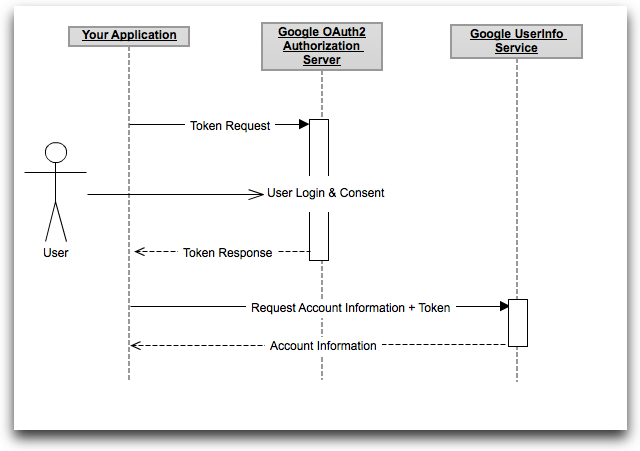
\includegraphics[width=\textwidth]{Bilder/googleOauth.png}
\label{fig:google_oauth}
\caption{Nutzungsbeispiel f\"ur \emph{OAuth}}
\end{figure}

Da wir unseren eigenen Account nutzen und die Daten nicht Sicherheitskritisch sind, haben
 wir die zweite Variante gew\"ahlt und authentifizieren uns bei jedem Service-Aufruf mit
 Username und Passwort.

\subsubsection{Kontakte suchen}
Die \emph{gdata}-Bibliothek bietet die Möglichkeit, Kontakte mit Angabe eines \emph{Querys}
 herunterzuladen.
Das \emph{Query} kann jedoch nur zwischen Gruppen unterscheiden, jedoch nicht nach anderen
 Kriterien wie z.\ B.\ dem Vornamen oder dem Nachnamen eines Kontakts filtern.

Das Suchen von Kontakten geschieht in unserem Projekt durch das Herunterladen aller Kontakte
 einer Gruppe und anschließendem sortieren "`von Hand"'.

\subsubsection{Kontakte einf\"ugen}
Das Einfügen von Kontakten ist über ein erstelltes Service-Objekt 